\subsection{Toy model}

Assume that we have two agents: Alice, a service provider, and Bob, a service requester. 
For a generic service, Bob will pay Alice $p$ each period.
The generic service will typically imply a requirement that the value of the funds involved in the service it itself `insured'.
For instance, Bob may enlist Alice to perform an atomic swap for funds of total value $V$, offering a payment $p$ for this service, where $p<V$.
Alice has options, as follows.

\begin{enumerate}
    \item[A:] post collateral $D$ upfront, such that $D=V$
    \item[B:] accrue collateral by saving payments $p$ each time period $t$
\end{enumerate}

The constraint is that Alice is not able to offer a service for a value larger than the sum of the collateral that she has in escrow. 
In the first case, Alice is able to offer a service of a value equal to the amount of posted collateral, $D$.
In the second case, the insured value is equal to the cumulative sum of the payments received.

While (A) offers users insurance of a larger transaction volume immediately, it involves a high capital burden on Alice, who must post collateral equal to the total value $V$. 
In contrast, (B) enables Alice to use the received payments $p$ as collateral, with the \textit{promise} that the sum of payments to Alice are sufficient to ensure full collateralization, previous payments will be made to Alice directly.
This eases the upfront collateral burden on Alice.

\begin{figure}
    \centering
    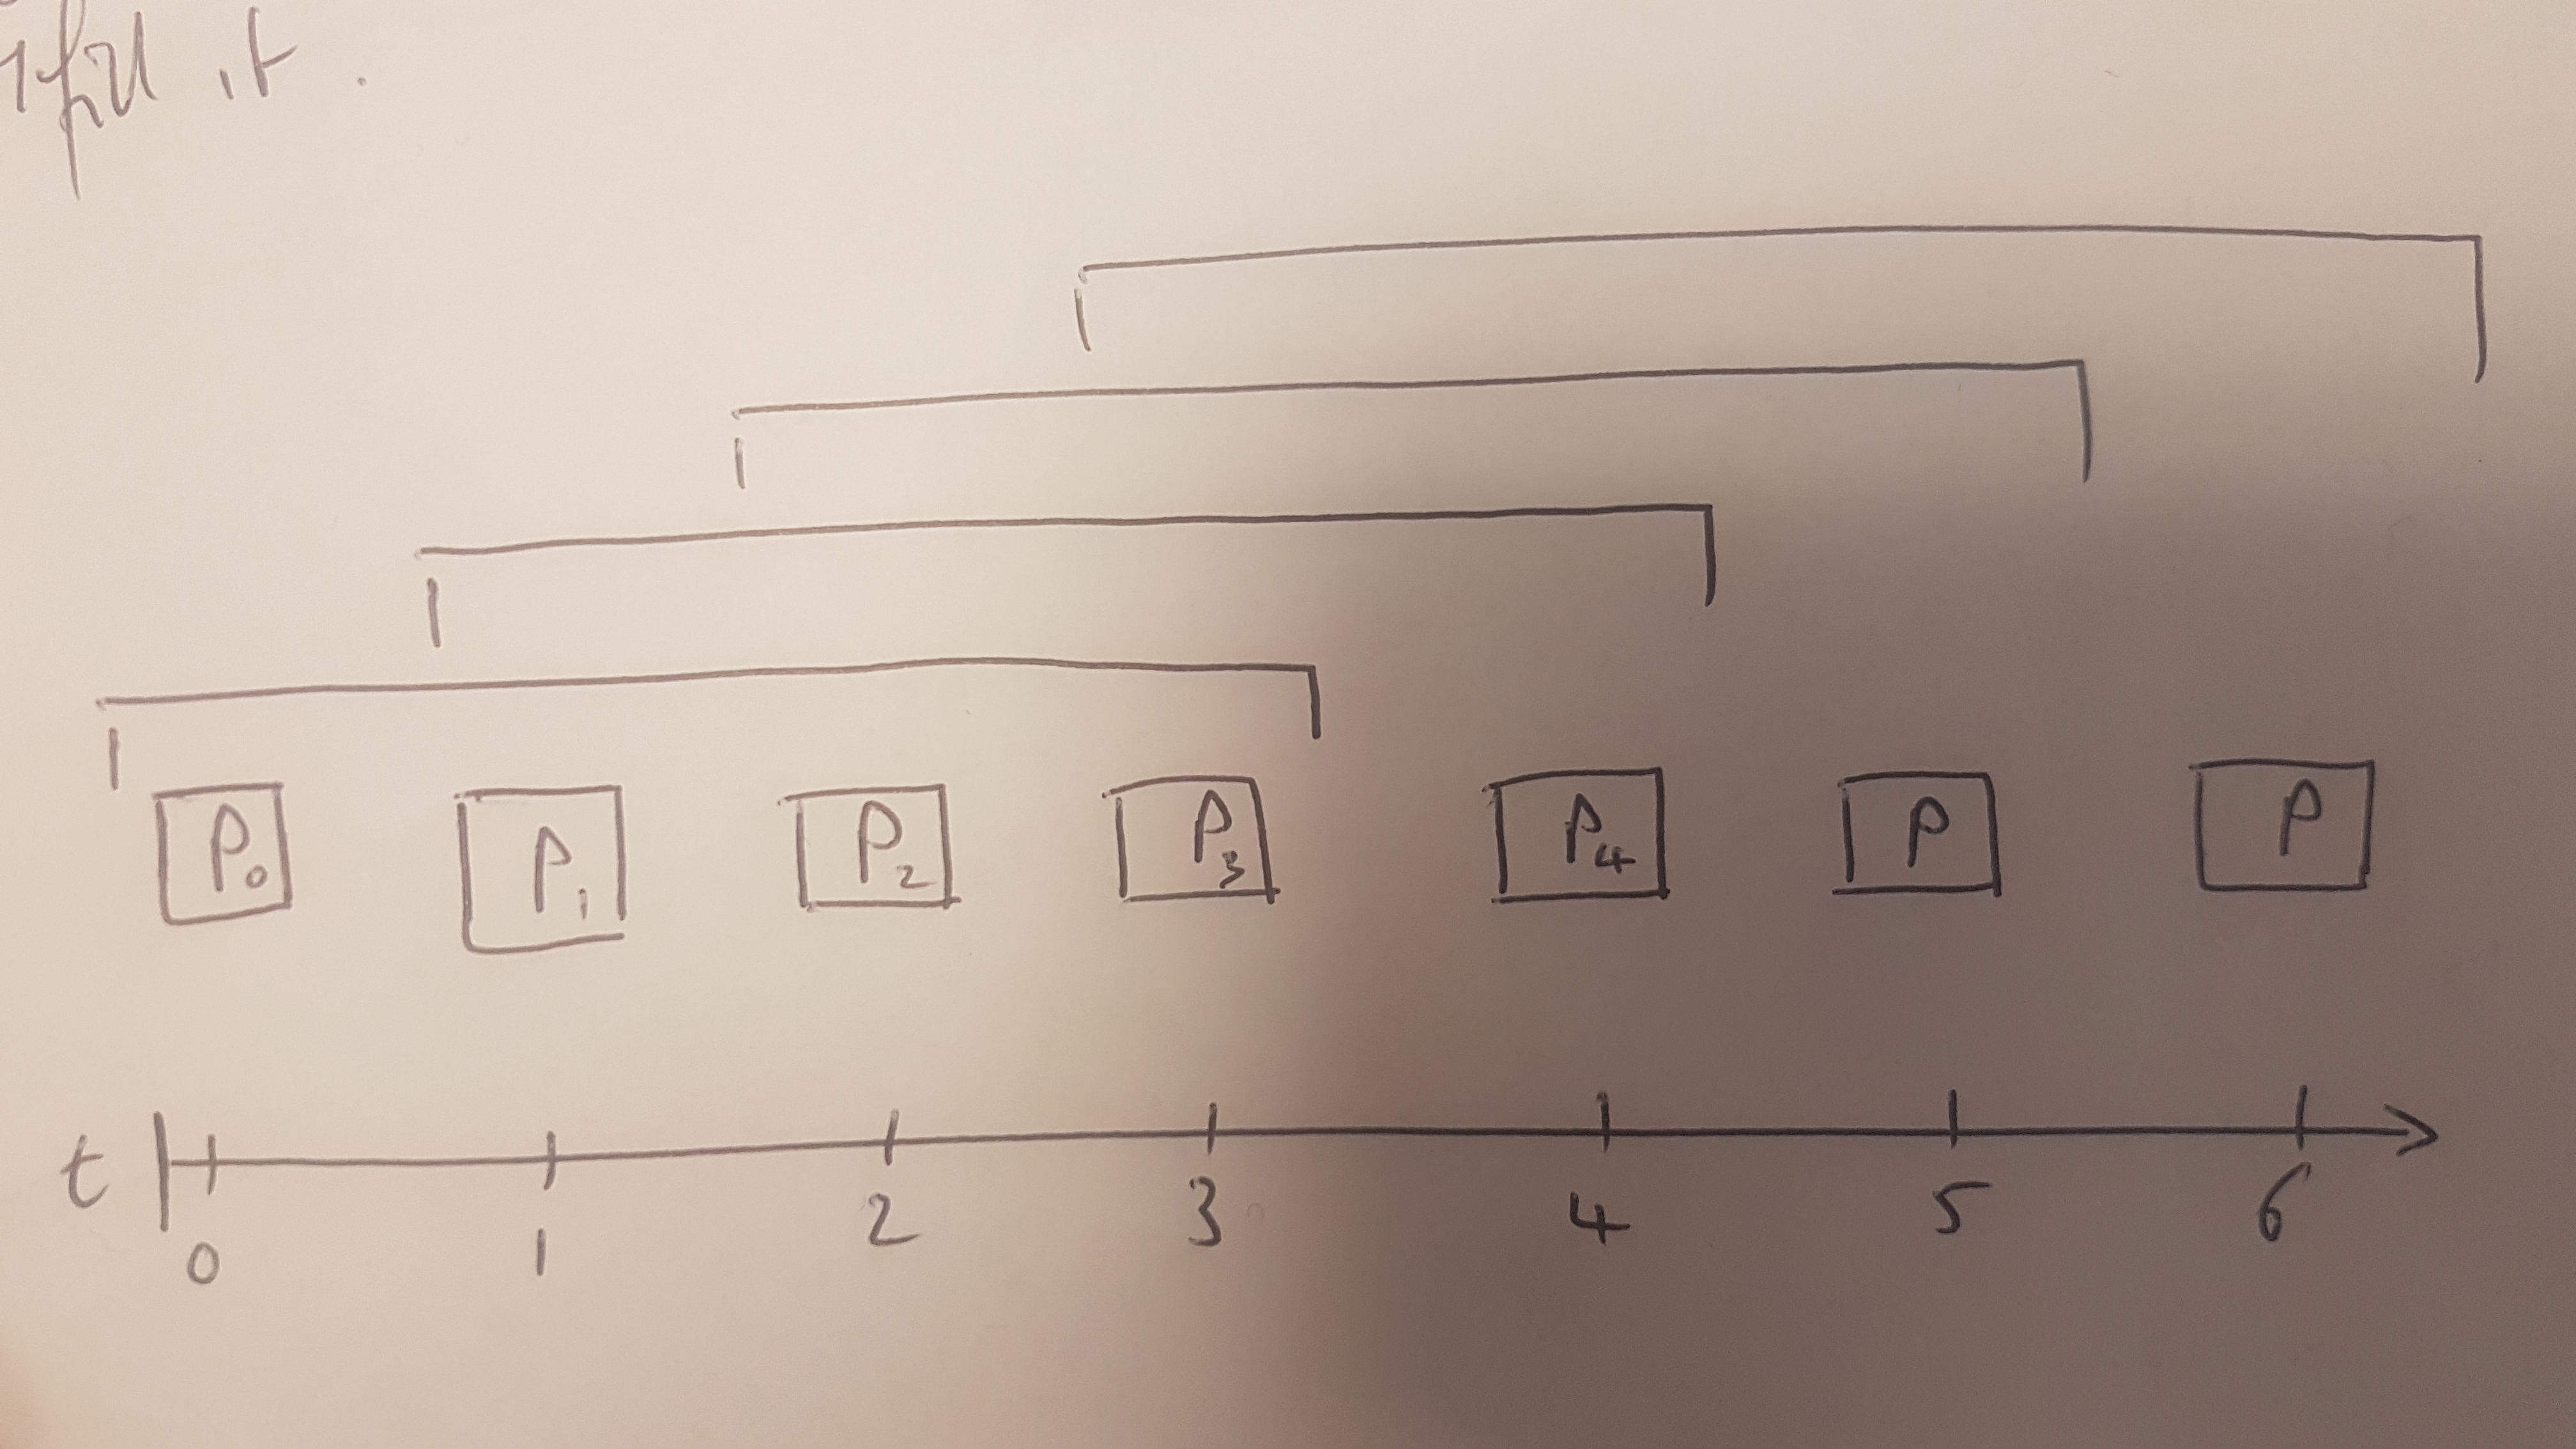
\includegraphics[width=\textwidth]{promise/figures/slidingwindows.jpg}
    \caption{Figure showing the mechanics of the sliding window.}
    \label{fig:slidingwindows}
\end{figure}

Alice decides to eventually offer collateral equivalent to $S=4$ periods of stored payments (from $t=0$ to $t=3$).
Therefore, until $t=4$, she does not receive any payment. 
At $t=4$, she receives payment $p$, which discounted is $(\frac{\delta}{1+r})^4$.
Similarly, at $t=5$, she receives another payment $p$, worth $(\frac{\delta}{1+r})^5$ to Alice today.
At the same time, Alice accrues opportunity costs of the locked funds ($p$) per period.
Alice incurs an opportunity cost of $\mathrm{E}[r]p$ in the first period, $\mathrm{E}[r](2p)(\frac{\delta}{1+r})$ in the second period, etc. 

If Alice offers such a service indefinitely, the total value of this, $T_v$, for a single iteration, is as follows. 

\begin{equation}
\label{eq:payoffs_longform}
T_v=(\frac{\delta}{1+r})p-\mathrm{E}[r](p+2p(\frac{\delta}{1+r})+3p(\frac{\delta}{1+r})^2+4p(\frac{\delta}{1+r})^3)
\end{equation}

Iterating $k$ times, the total net present value of $T_v$ is:

\begin{equation}
\label{eq:payoffs_longform}
T_v=\sum_{k=0}^{\infty}(\frac{\delta}{1+r})^{S+k}p-\mathrm{E}[r]p\sum_{k=0}^{\infty}(\frac{\delta}{1+r})^k(\sum_{i=0}^{S-1}(i+1)(\frac{\delta}{1+r})^i)
\end{equation}

\lgu{From here, maybe we want to compare to the status quo, where the operator fronts all the collateral upfront.
We would find that since the system `ramps up', the opportunity costs would be lower in the beginning, but this isn't that interesting because at the same time the service level is worse (only insured up to the cumulative total). So really what we are presenting is a funding model for cryptoeconomic protocols, where the operator's collateral is made up of user payments until some threshold cumulative total is reached? We could argue that this is valuable because it allows operators to get started?}

\dom{I agree with you. So in essence the cost of the locked collateral is reduced until you reach $t=4$ in the model above. Overall, it helps you bootstrap your system and allows your intermediaries to accumulate the required collateral. What I'm wondering is, if you have the same motivation to not cheat with the lower collateral in the beginning. I guess here we need to argue in a different way from the Balance paper. In Balance we say that $p=0$ and than argue that the proofs still hold. Here we need to assume that $p>0$ and perfect competition does not exist. This needs to go into the security discussion.}